\documentclass[tikz,border=12pt]{standalone}
\usepackage[T1]{fontenc}
\usepackage{mathpazo}
\usepackage{amsmath,amssymb}
\usetikzlibrary{arrows.meta, positioning, calc}

\definecolor{stblue}{HTML}{7B97AD}
\definecolor{rwgold}{HTML}{B8995E}
\definecolor{sage}{HTML}{7A9A7E}
\definecolor{dkbrown}{HTML}{3D3530}
\definecolor{wmgray}{HTML}{7B7067}
\definecolor{cream}{HTML}{F9F6F0}
\definecolor{border}{HTML}{D4C9B8}
\definecolor{terracotta}{HTML}{C47A6A}

\begin{document}
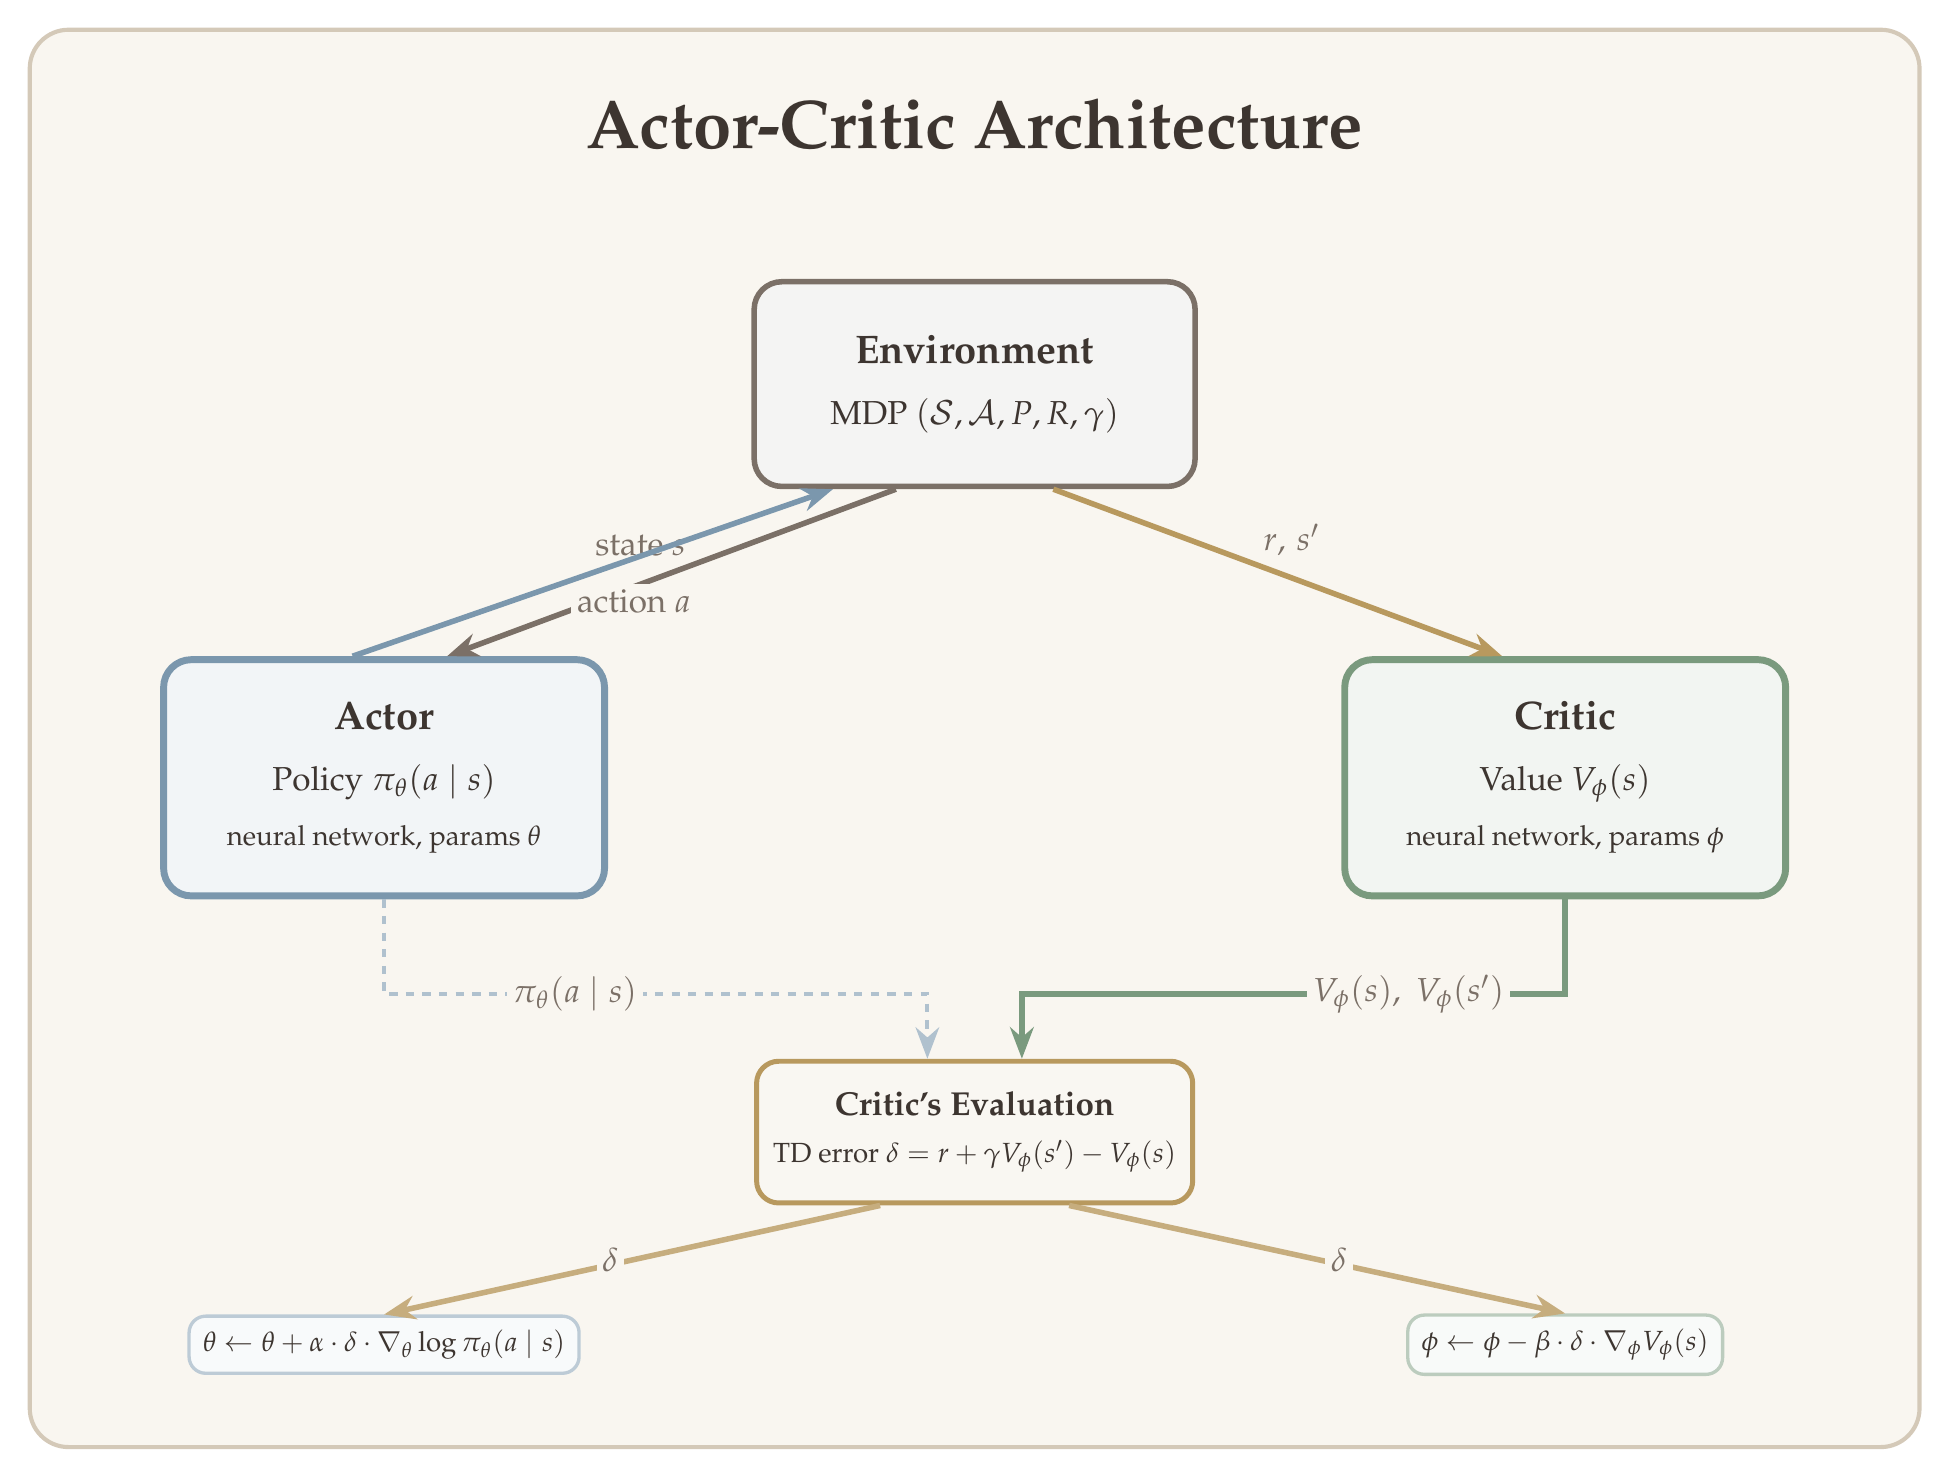
\begin{tikzpicture}[
  >={Stealth[length=4mm, width=3mm]},
  pbox/.style={
    draw=#1, line width=2.5pt, fill=#1!10, rounded corners=10pt,
    minimum width=56mm, minimum height=30mm, font=\Large, text=dkbrown,
    align=center, inner sep=8pt
  },
  sbox/.style={
    draw=#1, line width=1.8pt, fill=#1!8, rounded corners=8pt,
    minimum width=52mm, minimum height=18mm, font=\large, text=dkbrown,
    align=center, inner sep=6pt
  },
  arr/.style={->, line width=2pt, dkbrown},
  lbl/.style={font=\large, text=wmgray, align=center, fill=cream, inner sep=2pt},
]

% Background
\fill[cream, rounded corners=14pt] (-2,-10.5) rectangle (22,7.5);
\draw[border, rounded corners=14pt, line width=1.5pt] (-2,-10.5) rectangle (22,7.5);

% Title
\node[font=\Huge\bfseries, text=dkbrown] at (10,6.3)
  {Actor-Critic Architecture};

% =============================================
% Top: Environment
% =============================================
\node[draw=wmgray, line width=2pt, fill=wmgray!8, rounded corners=10pt,
      minimum width=56mm, minimum height=26mm,
      font=\Large, text=dkbrown, align=center, inner sep=8pt]
  (env) at (10,3)
  {\textbf{Environment}\\[4pt]
   {\large MDP $(\mathcal{S}, \mathcal{A}, P, R, \gamma)$}};

% =============================================
% Left: Actor (Policy)
% =============================================
\node[pbox=stblue] (actor) at (2.5,-2)
  {\textbf{Actor}\\[4pt]
   {\large Policy $\pi_\theta(a \mid s)$}\\[2pt]
   {\normalsize neural network, params $\theta$}};

% =============================================
% Right: Critic (Value)
% =============================================
\node[pbox=sage] (critic) at (17.5,-2)
  {\textbf{Critic}\\[4pt]
   {\large Value $V_\phi(s)$}\\[2pt]
   {\normalsize neural network, params $\phi$}};

% =============================================
% Bottom center: TD Error
% =============================================
\node[sbox=rwgold] (td) at (10,-6.5)
  {\textbf{Critic's Evaluation}\\[3pt]
   {\normalsize TD error $\delta = r + \gamma V_\phi(s') - V_\phi(s)$}};

% =============================================
% Bottom: Update rules
% =============================================
\node[draw=stblue!50, line width=1.2pt, fill=stblue!5, rounded corners=6pt,
      font=\normalsize, text=dkbrown, align=center, inner sep=5pt]
  (upd-actor) at (2.5,-9.2)
  {$\theta \leftarrow \theta + \alpha \cdot \delta \cdot \nabla_\theta \log \pi_\theta(a \mid s)$};

\node[draw=sage!50, line width=1.2pt, fill=sage!5, rounded corners=6pt,
      font=\normalsize, text=dkbrown, align=center, inner sep=5pt]
  (upd-critic) at (17.5,-9.2)
  {$\phi \leftarrow \phi - \beta \cdot \delta \cdot \nabla_\phi V_\phi(s)$};

% =============================================
% Arrows
% =============================================

% Environment -> Actor: state s (diagonal)
\draw[arr, wmgray] ([xshift=-10mm]env.south) -- ([xshift=8mm]actor.north)
  node[pos=0.45, lbl, above left] {state $s$};

% Actor -> Environment: action a (diagonal, offset from state arrow)
\draw[arr, stblue] ([xshift=-4mm]actor.north) -- ([xshift=-18mm]env.south)
  node[pos=0.45, lbl, below right] {action $a$};

% Environment -> Critic: reward r, next state s' (diagonal)
\draw[arr, rwgold] ([xshift=10mm]env.south) -- ([xshift=-8mm]critic.north)
  node[pos=0.45, lbl, above right] {$r,\, s'$};

% Critic -> TD box (down and right-to-center)
\draw[arr, sage] (critic.south) -- ++(0,-1.2) -| ([xshift=6mm]td.north)
  node[pos=0.25, right, lbl, xshift=4pt] {$V_\phi(s),\; V_\phi(s')$};

% Actor info -> TD box (dashed, down and left-to-center)
\draw[->, line width=1.5pt, dashed, stblue!60]
  (actor.south) -- ++(0,-1.2) -| ([xshift=-6mm]td.north)
  node[pos=0.25, left, lbl, xshift=-4pt] {$\pi_\theta(a \mid s)$};

% TD -> update rules
\draw[arr, rwgold!80] ([xshift=-12mm]td.south) -- (upd-actor.north)
  node[midway, left, lbl, xshift=-2pt] {$\delta$};
\draw[arr, rwgold!80] ([xshift=12mm]td.south) -- (upd-critic.north)
  node[midway, right, lbl, xshift=2pt] {$\delta$};

\end{tikzpicture}
\end{document}
